\documentclass[10pt,tikz,border=5pt]{standalone}
\usepackage[T1]{fontenc}
\usepackage{lmodern,amsmath,booktabs,array,tabularx,microtype,tikz}
\usetikzlibrary{patterns,patterns.meta,shapes.geometric,arrows.meta,calc,positioning}
\begin{document}
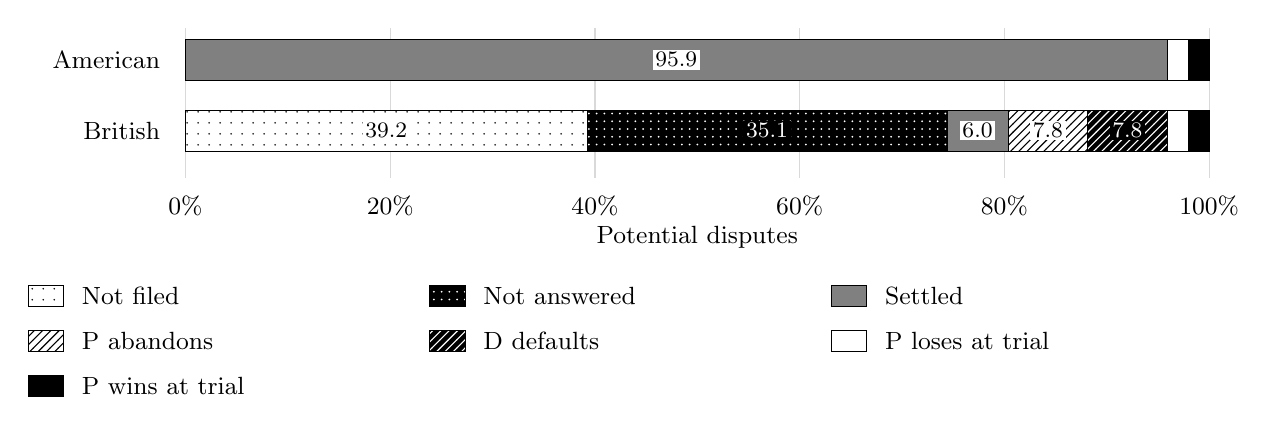
\begin{tikzpicture}[font=\small]
\draw[black!15] (2.0,.5)--(2.0,2.4);
\node[anchor=north] at (2.0,.4) {0\%};
\draw[black!15] (4.6,.5)--(4.6,2.4);
\node[anchor=north] at (4.6,.4) {20\%};
\draw[black!15] (7.2,.5)--(7.2,2.4);
\node[anchor=north] at (7.2,.4) {40\%};
\draw[black!15] (9.8,.5)--(9.8,2.4);
\node[anchor=north] at (9.8,.4) {60\%};
\draw[black!15] (12.4,.5)--(12.4,2.4);
\node[anchor=north] at (12.4,.4) {80\%};
\draw[black!15] (15.0,.5)--(15.0,2.4);
\node[anchor=north] at (15.0,.4) {100\%};
\node[anchor=east] at (1.8,2.0) {American};
\path[fill=black!50,draw=black,line width=.25pt] (2.00000000,1.74) rectangle (14.46693500,2.26);
\node[text=black,fill=white,font=\footnotesize,inner sep=1pt] at (8.23346750,2.0) {95.9};
\path[fill=white,draw=black,line width=.25pt] (14.46693500,1.74) rectangle (14.73347660,2.26);
\path[fill=black,draw=black,line width=.25pt] (14.73347660,1.74) rectangle (15.00000520,2.26);
\node[anchor=east] at (1.8,1.1) {British};
\path[preaction={fill=white,draw=none},pattern={Dots[distance=4pt,radius=.35pt]},pattern color=black,draw=black,line width=.25pt] (2.00000000,0.8400000000000001) rectangle (7.10133000,1.36);
\node[text=black,fill=white,font=\footnotesize,inner sep=1pt] at (4.55066500,1.1) {39.2};
\path[preaction={fill=black,draw=none},pattern={Dots[distance=2.8pt,radius=.35pt]},pattern color=white,draw=black,line width=.25pt] (7.10133000,0.8400000000000001) rectangle (11.66933500,1.36);
\node[text=white,fill=black,font=\footnotesize,inner sep=1pt] at (9.38533250,1.1) {35.1};
\path[fill=black!50,draw=black,line width=.25pt] (11.66933500,0.8400000000000001) rectangle (12.44818710,1.36);
\node[text=black,fill=white,font=\footnotesize,inner sep=1pt] at (12.05876105,1.1) {6.0};
\path[preaction={fill=white,draw=none},pattern=north east lines,pattern color=black,draw=black,line width=.25pt] (12.44818710,0.8400000000000001) rectangle (13.45754740,1.36);
\node[text=black,fill=white,font=\footnotesize,inner sep=1pt] at (12.95286725,1.1) {7.8};
\path[preaction={fill=black,draw=none},pattern=north east lines,pattern color=white,draw=black,line width=.25pt] (13.45754740,0.8400000000000001) rectangle (14.46692590,1.36);
\node[text=white,fill=black,font=\footnotesize,inner sep=1pt] at (13.96223665,1.1) {7.8};
\path[fill=white,draw=black,line width=.25pt] (14.46692590,0.8400000000000001) rectangle (14.73346750,1.36);
\path[fill=black,draw=black,line width=.25pt] (14.73346750,0.8400000000000001) rectangle (14.99999610,1.36);
\node at (8.5,-.25) {Potential disputes};
\path[preaction={fill=white,draw=none},pattern={Dots[distance=4pt,radius=.35pt]},pattern color=black,draw=black,line width=.25pt] (0.0,-1.13) rectangle (0.45,-0.87);
\node[anchor=west] at (0.56,-1.0) {Not filed};
\path[preaction={fill=black,draw=none},pattern={Dots[distance=2.8pt,radius=.35pt]},pattern color=white,draw=black,line width=.25pt] (5.1,-1.13) rectangle (5.55,-0.87);
\node[anchor=west] at (5.66,-1.0) {Not answered};
\path[fill=black!50,draw=black,line width=.25pt] (10.2,-1.13) rectangle (10.649999999999999,-0.87);
\node[anchor=west] at (10.76,-1.0) {Settled};
\path[preaction={fill=white,draw=none},pattern=north east lines,pattern color=black,draw=black,line width=.25pt] (0.0,-1.6999999999999997) rectangle (0.45,-1.44);
\node[anchor=west] at (0.56,-1.5699999999999998) {P abandons};
\path[preaction={fill=black,draw=none},pattern=north east lines,pattern color=white,draw=black,line width=.25pt] (5.1,-1.6999999999999997) rectangle (5.55,-1.44);
\node[anchor=west] at (5.66,-1.5699999999999998) {D defaults};
\path[fill=white,draw=black,line width=.25pt] (10.2,-1.6999999999999997) rectangle (10.649999999999999,-1.44);
\node[anchor=west] at (10.76,-1.5699999999999998) {P loses at trial};
\path[fill=black,draw=black,line width=.25pt] (0.0,-2.2699999999999996) rectangle (0.45,-2.01);
\node[anchor=west] at (0.56,-2.1399999999999997) {P wins at trial};
\end{tikzpicture}\end{document}